\chapter{양면 시장 이론}\label{cha:twosidedmarketheory}

\section*{학습개요}
플랫폼 경제를 설명하는 대표적인 경제 이론은 다면 시장 이론이다. 이 강의에서는 그 중 가장 단순한 구조인 양면시장이론(two-sided market theory)을 학습한다.


\section*{학습목표}
\begin{enumerate}
\item 양면 시장의 정의를 설명할 수 있다.
\item 양면 시장에서의 시소 원칙을 설명할 수 있다.
\item 플랫폼의 회원제 요금과 사용량 연동 요금을 구별할 수 있다.
\item 수요의 가격 탄력성에 따라 플랫폼이 이윤을 극대화 할 수 있는 전략을 설명할 수 있다.
\item 주어진 상황에 따라 하나의 플랫폼만 사용하는 것과 다수의 플랫폼만 사용하는 것의 관계를 설명할 수 있다.
\end{enumerate}

\section*{주요 용어}
양면 시장, 시소 원칙, 수요의 가격 탄력성, 하나의 플랫폼 사용(single-homing), 다수의 플랫폼 사용(multi-homing), 병목을 향한 경쟁

\pagebreak

\section{양면 시장의 정의}\label{sec:}
\begin{itemize}
\item 가격 구조를 강조한 정의 \cite[pp. 664--665]{Rochet:2006jl} $\rightarrow$ 반독점 규제와 연결됨
	\begin{quote}
	``플랫폼이 동일한 양에 대해 시장의 한 면에 더 높은 가격을 부과하고 다른 면에는 낮은 가격을 부과함으로써, 거래량에 영향을 줄 수 있을 때 양면 시장이라고 할 수 있다. 즉, 가격 구조가 중요하고, 플랫폼은 양면 모두가 플랫폼에 머물러 있도록 가격 구조를 설계할 수 있어야만 한다.  만약 어느 최종 사용자가 실제 할당된 짐을 받아들이지 않고 떠날 수 있다면 단면 시장이다\footnote{A market if two-sided if the platform can affect the volume of transactions by charging more to one side of the market and reducing the price paid by the other side by an equal amount; in other words, the price structure matters, and platforms must design it so as to bring both sides on board. The market is one-sided if the end-users negotiate away the actual allocation of the burden.}."
	\end{quote}
	\begin{itemize}
	\item 두 종류의 사용자 집단 
		\begin{itemize}
		\item 거래 중개를 위해 플랫폼이 필요
		\item 플랫폼은 재화나 서비스를 두 사용자에게 동시에 제공
		\end{itemize}
	\item 두 집단 간의 간접적인 외부성
		\begin{itemize}
		\item 어느 한 면의 사용자 수가 증가하면, 다른 면의 사용자에게 이득이 발생
		\item 이 두 가지 특성만 생각하면, 직접 거래를 제외한 일상의 거의 모든 거래는 어느 정도 양면 시장의 속성을 가짐
		\item 하지만, 양면 시장이라고 부를 수 있는 독특한 특징은 다음의 가격 구조
		\end{itemize}
	\item 비대칭적인 가격 구조
		\begin{itemize}
		\item 어느 한 면의 가격을 높이고 다른 한 면의 가격을 낮추기 때문
		\item 양면 모두가 플랫폼에 참여하도록 설계해야 함
		\item 동시에, 즉 양면 모두가 자신의 요금 체계를 받아들여야 함
		\end{itemize}
	\end{itemize}
\end{itemize}

\pagebreak

\section{양면 시장의 가격 결정}
\begin{itemize}
\item 가격 구조에 관한 질문
	\begin{enumerate}
	\item 가격 구조에 영향을 미치는 요소는 무엇인가? 
		\begin{itemize}
		\item \cite{Rochet:2006jl}, 시소 원칙(the Seesaw principle)
			\begin{itemize}
			\item 플랫폼의 이윤을 높이도록 A면에 높은 가격을 부과하게 하는 요인은, 더 높은 이윤을 얻고자 B면의 사용자를 유인하기 위해 B면의 가격을 낮추도록 할 수 있음
			\end{itemize}
		\item \href{https://news.naver.com/main/read.nhn?mode=LSD&mid=sec&sid1=105&oid=143&aid=0000044770}{김준엽, 2006, ``소니 PS3 1대 팔때마다 22만원씩 밑진다", 국민일보 2006.11.20.}	
			\begin{itemize}
			\item 게임 이용자 -- 콘솔 게임기 판매사 -- 게임 개발사
			\item  $\rightarrow$ 게임 이용자가 지불할 가격을 낮추면, 
			\item $\rightarrow$ 게임 이용자의 콘솔 게임기 수요와 게임 수요를 모두 늘릴 수 있음
			\item $\rightarrow$ 게임 개발사로부터의 로열티를 높일 수 있음
			\end{itemize}

				\begin{table}[htp]
				\begin{center}
				\begin{threeparttable}
				\caption{플랫폼 가격 전략의 예}
				\label{tab:moneyandsubsidysidesforcommonmultisdedplatformindustries}
				\begin{tabularx}{\textwidth}{lll}
				\toprule
				플랫폼 & A 면 & B면 \\
				\midrule
				콘솔 게임기 & 소비자는 한계 비용 또는  & 게임 개발사로부터 로열티를 받음 \\
				& 그 이하의 가격으로 콘솔 게임기를 구입 &   \\
				TV 방송 & 시청자의 지불은 없음 & 광고주로부터 광고비를 받음  \\
				신용카드 & 소비자의 지불은 없음,   & 가맹점으로부터 거래 수수료를 받음 \\
				& 마일리지, 포인트 등을 받기도 함 & \\
				쇼핑몰 & 소비자의 지불은 없음, & 판매점으로부터 임대료를 받음 \\
				& 무료 주차나 이벤트 등의 보상이 있기도 함 & \\
				온라인 쇼핑몰 & 소비자의 지불은 보통 없음  & 판매자가 수수료를 지불\\
				\bottomrule
				\end{tabularx}
				\begin{tablenotes}
				\small
				\item 출처: \cite{Evans:2017uw}, 표 2-1.
				\end{tablenotes}
				\end{threeparttable}
				\end{center}
				\end{table}%
			
		\end{itemize}

\pagebreak
		
	\item 플랫폼이 설계할 수 있는 가격 구조는 무엇인가?
		\begin{itemize}
		\item  전체 서비스에 대한 구독 요금을 지불 $\rightarrow$ 회원제 요금
		\item 매 거래마다 요금을 지불 $\rightarrow$ 사용량 연동 요금
		\item 이 두 방법이 상호 배타적이지는 않음
			\begin{itemize}
			\item	 즉, 동시에 존재하는 요금제도 있음
			\item 디지털 콘텐츠의 정기 구독 $+$ 특정 콘텐츠는 개별 구매
			\end{itemize}
		\end{itemize}
	\end{enumerate}
\item 두 가지 질문 모두와 관련하여, 현실적으로 중요한 이슈는 고려 대상이 되는 면에서의 수요의 가격 탄력성 \cite[pp. 129--130]{Rysman:2009aa}
	\begin{itemize}
	\item A 면의 가격 탄력성이 매우 높고, B 면의 가격 탄력성이 높지 않다면
	\item A 면에 한계비용보다 낮은 가격을 부과하여 더 많은 소비자를 유인하고, B 면은 한계비용보다 더 높은 가격을 부과(a higher mark-up pricing)할 수 있음
	\end{itemize}		
\item $\rightarrow$ 만약 A 면의 소비 증가로 B 면의 사용자를 더 유인할 수 있다면(즉, 간접적인 네트워크 효과가 있다면), 플랫폼은 양면 모두에서 이윤을 얻을 수 있음	
	\begin{itemize}
	\item 플랫폼은 A면 (왼쪽 그래프)과 B면(오른쪽 그래프) 모두를 상대

		\begin{figure}[htbp]
		\begin{center}
		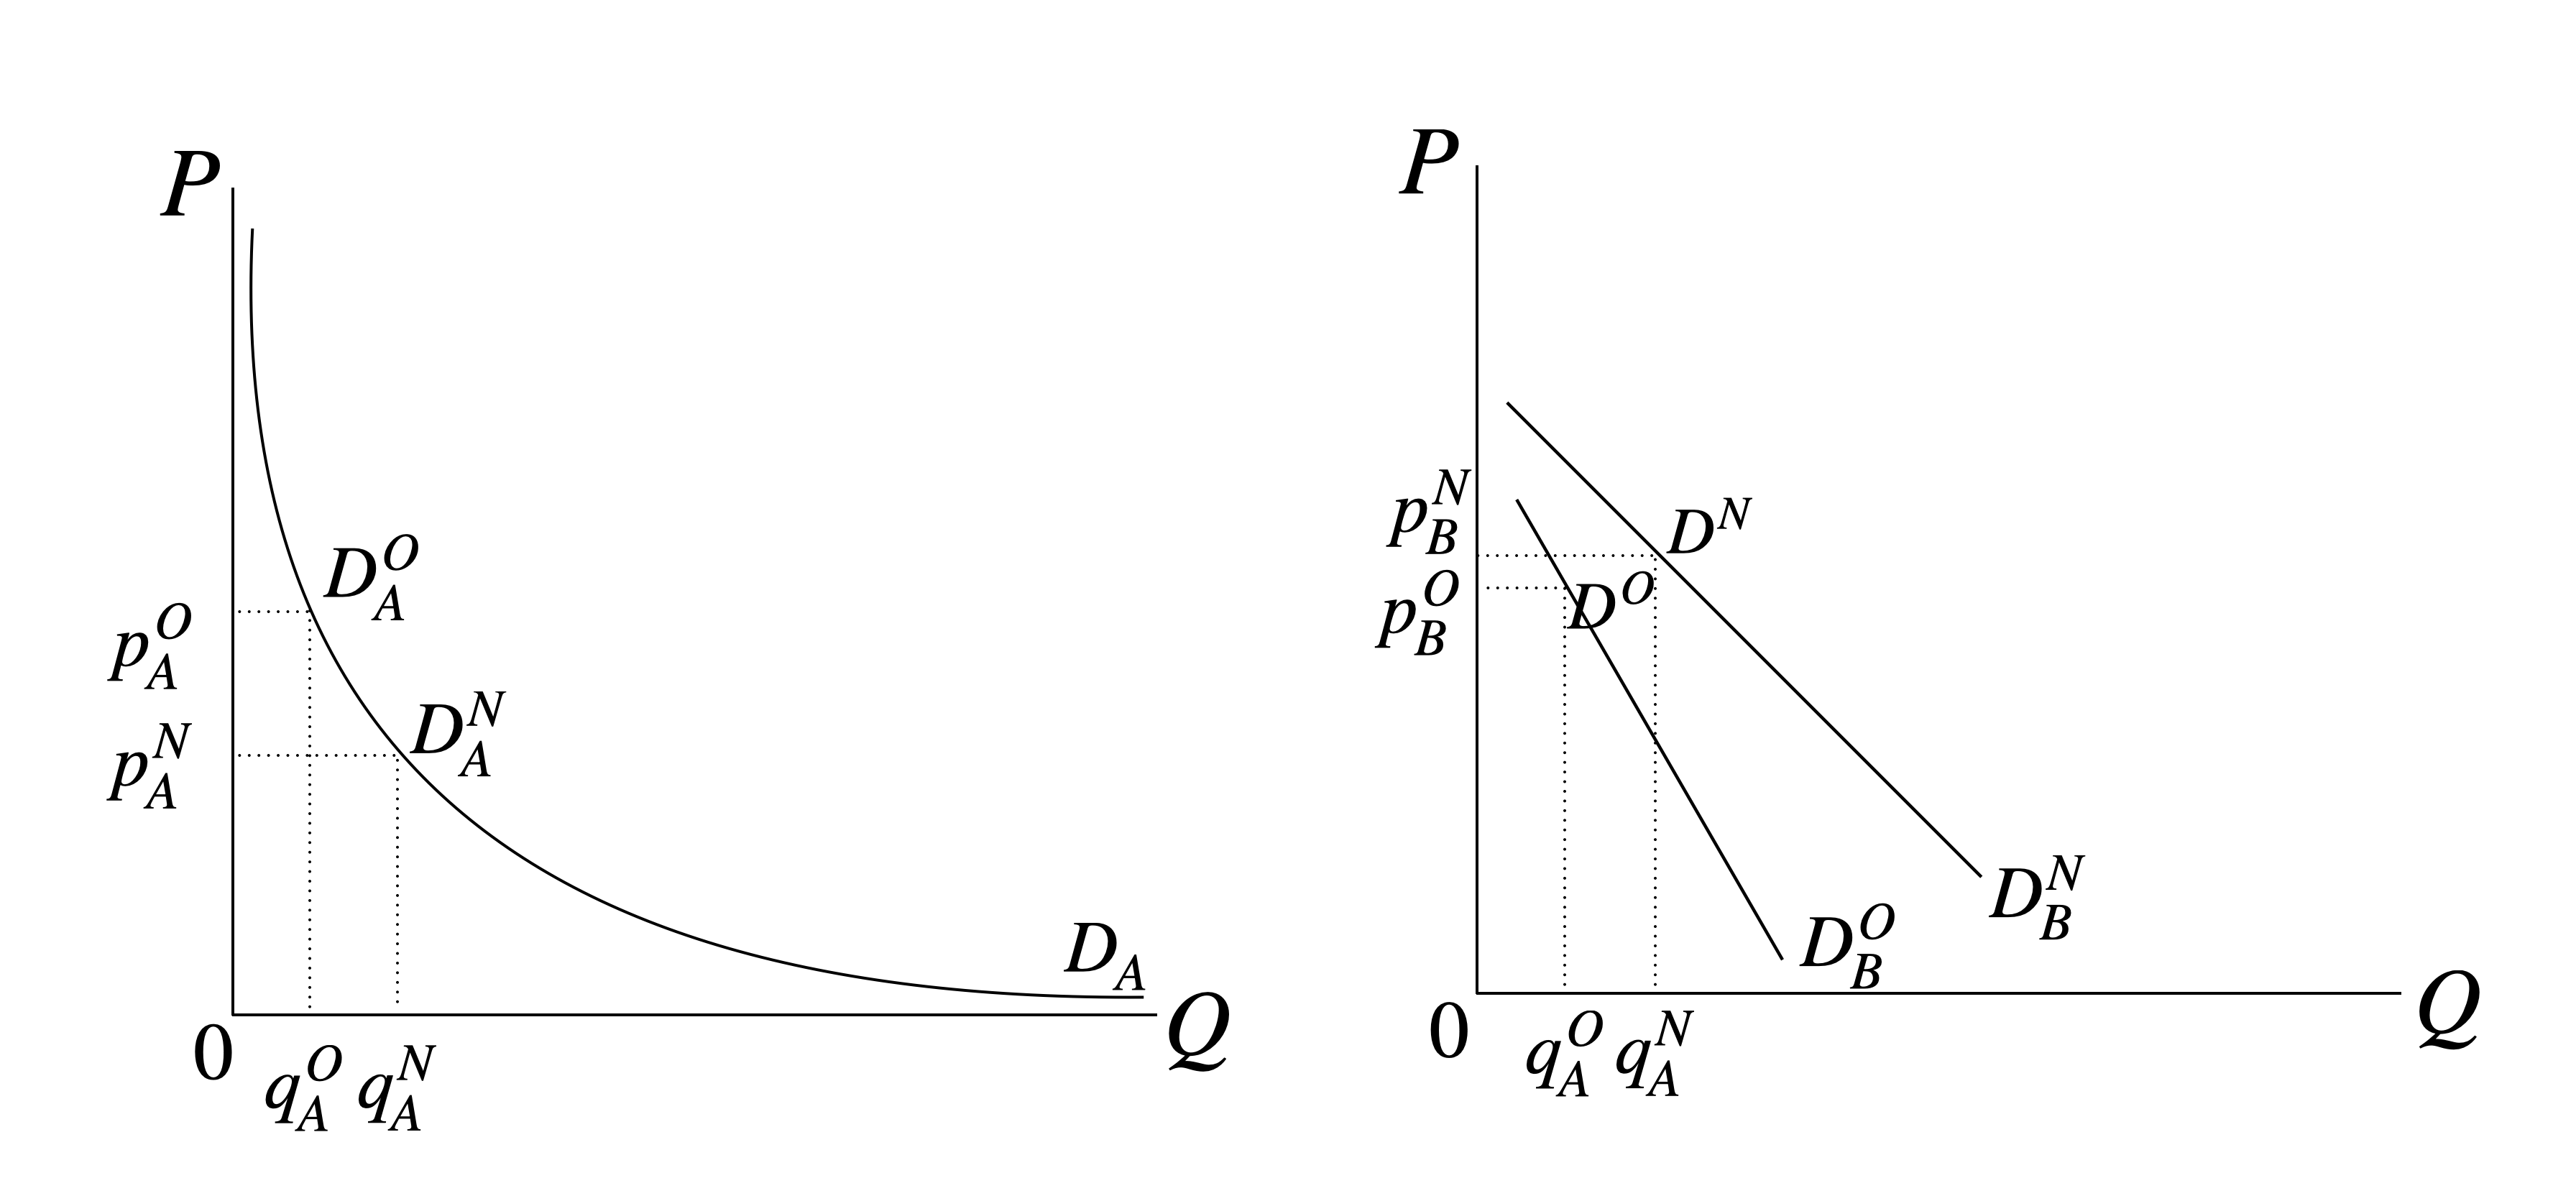
\includegraphics[scale=0.2]{two-sided-market-pricing.png}
		\caption{양면 시장의 가격 구조}
		\label{fig:two-sided-market-pricing}
		\end{center}
		\end{figure}
	
	\item 플랫폼이 A 면의 가격을 낮추면 ($p_{A}^{O} > p_{A}^{N}$), 수요량은 증가 ($q_{A}^{O} < q_{A}^{N} $)
		\begin{itemize}
		\item 수요량이 충분히 늘어나면, 수입이 증가 ($p_{A}^{O} q_{A}^{O} = \pi_{A}^{O} < \pi_{A}^{N} = p_{A}^{N} q_{A}^{N}$) 
		\end{itemize}
	\item 그리고, A 면의 수요량 증가로, B 면의 수요가 늘어나면 ($D_{B}^{O} \rightarrow D_{B}^{N}$)
	\item B 면에서 가격을 높여도 ($p_{B}^{O} < p_{B}^{N} $)
		\begin{itemize}
		\item 수입이 증가 ($p_{B}^{O} q_{A}^{O} = \pi_{B}^{O} < \pi_{B}^{N} = p_{B}^{N} q_{A}^{N}$)
		\item 즉, B면에서 사각형 $p_{B}^{O}0q_{A}^{O}D^{O}$의 면적보다 사각형 $p_{B}^{N}0q_{A}^{N}D^{N}$의 면적이 더 크다는 의미, A면도 마찬가지
		\end{itemize}
	\item 사각형 면적을 결정하는 것은 A면과 B면의 가격에 대한 수요 탄력성	
	\end{itemize}
\item $\rightarrow$ 플랫폼은 어느 한 면의 가격을 낮추고($\downarrow$), 다른 한 면의 가격을 높임으로써($\uparrow$) 이윤을 극대화 할 수 있음: 시소 원칙	
\end{itemize}




\section{하나의 플랫폼 사용 대 다수의 플랫폼 사용}
\begin{itemize}
\item 이 장에서는 플랫폼 간의 경쟁이 있을 때의 문제만 다룸
	\begin{itemize}
	\item 하나의 플랫폼 사용(single homing) 대 다수의 플랫폼 사용(multihoming)
	\end{itemize}
\item 다른 장에서 다룰 문제들
	\begin{itemize}
	\item 플랫폼에 사용자를 어떻게 모을 것인가? %$\rightarrow$ \ref{cha:networktheory}장과 \ref{cha:chikenandeggproblem}장
	\item 과세(taxation) %$\rightarrow$ \ref{cha:taxation}장
	\item 시장 구조(market structure)와 경쟁 정책(competition policy) %$\rightarrow$ \ref{cha:competitionpolicy}장
	\end{itemize}
\item 다수의 플랫폼을 사용하는 이유는 다양
	\begin{enumerate}
	\item 플랫폼의 상호 연결성이 없을 때, 각 플랫폼 마다의 네트워크 외부성을 누리기 위해,
	\item 매칭 확률을 높이기 위해,
	\item 독점 콘텐츠가 있을 때 등
	\end{enumerate}
\item $\rightarrow$ 결국, 어느 한 면의 사용자가 다수의 플랫폼을 사용하면 사용할 수록, 다른 한 면의 사용자가 한 개 이상의 플랫폼을 사용할 유인은 낮아짐
	\begin{itemize}
	\item $\rightarrow$ 어느 한 면은 다수의 플랫폼을 사용하지만, 다른 한 면은 하나의 플랫폼을 사용하는 방향으로 수렴
		\begin{itemize}
		\item 가맹점은 여러 개의 신용카드를 받아들이지만, 소비자는 한 두 개의 신용카드만 사용
		\end{itemize}
	\end{itemize}
\item $\rightarrow$ 어떤 면의 사용자가 하나의 플랫폼만 사용한다면
	\begin{itemize}
	\item 다른 면의 사용자는 하나의 플랫폼을 이용하는 이 사용자에게 접근하기 위해 더 많은 비용을 지불할 의사가 있을 것
		\begin{itemize}
		\item 이 소비자에게 독점 가격을 부과할 수 있기 때문
		\end{itemize}
	\item 따라서, 하나의 플랫폼 사용자를 만들기 위한 플랫폼 간 경쟁이 발생
		\begin{itemize}
		\item $\rightarrow$ 병목을 향한 경쟁(competitive bottleneck)
		\item[예)] 신용카드 사는 가맹점보다 카드 소비자를 더 고려 (마일리지 프로그램 등)
		\item $\rightarrow$ 상대적으로 다수의 플랫폼을 이용하는 사용자는 하나의 플랫폼을 이용하는 사용자보다 더 높은 가격을 지불
		\end{itemize}
	\end{itemize}
\item 최근의 이론은 앞의 논의와 반대로, 다수의 플랫폼 사용자가 하나의 플랫폼 사용자보다 더 낮은 가격을 지불할 수 있는 상황을 보여줌 \citep{Belleflamme:2019ts}
	\begin{itemize}
	\item 어떤 플랫폼의 사용자가 다른 플랫폼을 사용하는 선택이 아니라 시장을 벗어나는 선택을 한다면, 
	\item $\rightarrow$ 이 사용자가 지불할 가격을 낮추는 것이 유리할 수 있음
	\item 시장에는 두 개의 힘이 작동하고 있기 때문
		\begin{itemize}
		\item 시장 점유율을 높이기 위해 독점 가격보다 낮은 가격을 제시하는 플랫폼 간의 경쟁도 있지만,
		\item 가격에 민감하여 소비를 포기하는 소비자를 붙잡아 두기 위한 플랫폼 간의 경쟁도 있음
		\end{itemize}
	\end{itemize}
\item 가격 이외 다수의 플랫폼 사용을 줄이는 요소들
	\begin{enumerate}
	\item 독점 계약 $\rightarrow$ 독점 계약을 맺은 다른 면의 사용자가 있는 하나의 플랫폼을 사용할 것
	\item 호환성 $\rightarrow$ 호환성을 높이면, 다수의 플랫폼을 사용할 유인이 없음 $\rightarrow$ 만약, 플랫폼이 완전히 호환되고, 네트워크 효과를 내부화할 수 없다면, 플랫폼을 이용하도록 하려는 보조금의 유인 효과는 사라짐
	\end{enumerate}
\end{itemize}


\pagebreak

\section*{정리하기}
\begin{enumerate}
\item 양면 시장의 중요한 특징으로 (1) 플랫폼이 두 개 이상의 사용자 집단의 거래를 중개하는 것 (2) 이 집단 간에는 간접적인 외부성이 있다는 것 (3) 비대칭적인 가격 구조를 꼽을 수 있다.
\item 양면 시장의 시소 원칙은 플랫폼 사업자가 이윤을 높이기 위해 어느 한 면에 높은 가격을 부과하고, 다른 한 면의 가격을 낮추도록 할 수 있음을 의미한다. 이는 가격을 낮추어 사용자를 유인할 수 있기 때문에 그렇다.
\item 플랫폼의 가격 구조로는 (1) 전체 서비스에 대한 구독 요금을 받는 회원제 요금이나 (2) 매 거래마다 요금을 받는 사용량 연동 요금제가 대표적이다. 이 두 요금제는 서로 배타적이지는 않아 함께 사용될 수도 있다.
\item 양면의 수요탄력성에 따라 한 면의 가격을 낮추더라도 플랫폼 기업의 수입이 증가할 수 있고, 낮아진 가격으로 늘어난 수요량에 대응해 다른 면의 수요가 증가하면 역시 수입이 증가하여, 양면에서 모두 수입이 늘어나는 것도 가능하다.
\item 다수의 플랫폼을 사용하는 이유는 (1) 플랫폼 간 연결이 없을 때, 각 플랫폼 마다의 네트워크 외부성을 누리기 위해 (2) 매칭 확률을 높이기 위해 (3) 특정 플랫폼의 독점 콘텐츠가 있을 때 등이 대표적이다.
\item 어느 한 면의 사용자가 다수의 플랫폼을 사용하면 사용할 수록, 다른 한 면의 사용자는 하나의 플랫폼만 사용하게될 가능성이 높다.
\item 어느 한 면의 사용자가 하나의 플랫폼만 사용하면 이 사용자에게 독점 가격을 부과할 수 있으므로, 하나의 플랫폼 사용자를 만들기 위한 경쟁이 나타날 수 있다. 그 결과 상대적으로 다수의 플랫폼을 이용하는 사용자가 하나의 플랫폼을 이용하는 사용자에 비해 높은 가격을 지불하게 될 수 있다.
\item 하지만, 사용자가 다른 플랫폼을 사용하는 선택이 아니라 시장을 벗어나는 선택을 할 수 있다면, 오히려 사용자를 시장에 머물러 있을 수 있도록 하는 것이 유리할 수 있고 이 경우 다수의 플랫폼 사용자가 하나의 플랫폼 사용자보다 더 낮은 가격을 지불할 수도 있다.
\item 가격 이외에 하나의 플랫폼만 사용하도록 만드는 요소는 독점 계약, 호환성 등을 꼽을 수 있다.
\end{enumerate}

%\item \cite{Jullien:2012aa}
%\item 모형
%	\begin{itemize}
%	\item S (편의상, 판매자), B (구매자), 플랫폼
%	\item $t_{s}$: 거래 당 판매자가 플랫폼에 지불하는 수수료 $\rightarrow$ 수수료가 높아질 수록 판매자가 플랫폼을 통해하려는 거래 $D_{s}$는 줄어들 것: $D_{s}(t_{s})$
%	\item $t_{b}$: 거래 당 구매자가 플랫폼에 지불하는 수수료 $\rightarrow$ 수수료가 높아질 수록 구매자가 플랫폼을 통해하려는 거래 $D_{b}$는 줄어들 것: $D_{b}(t_{b})$
%	\item 플랫폼: 판매자와 구매자를 연결시켜 줌(매칭,  matching)
%	\item 플랫폼을 통한 총 거래: 각각 수요의 곱(product)으로 표현 $D_{b}(t_{b})D_{s}(t_{s})$
%	\item 플랫폼의 수입: $t_{b}+t_{s}$
%	\item 플랫폼의 비용: $c$
%	\item 플랫폼의 이윤 극대화 조건: $t_{b} + t_{s} - c = -\dfrac{D_{b}(t_{b})}{D_{b}^{'}(t_{b})} = -\dfrac{D_{s}(t_{s})}{D_{s}^{'}(t_{s})}$
%		\begin{itemize}
%		\item 정리하면,  $t_{i} - ( c - t_{j}) = -\dfrac{D_{i}(t_{i})}{D_{i}^{'}(t_{i})}$
%		\end{itemize}
%	\end{itemize}


%\section{양면시장 전략}
%\subsection{가격}
%\begin{itemize}
%\item 시장 A, B의 양면이 있을 때, 플랫폼 이용의 가격은 A 시장의 수요와 비용 뿐만 아니라, A 시장의 결과가 B 시장에 미치는 영향과 그로 인한 B 시장에서의 이윤 변화에 영향을 받음
%\item 플랫폼은 어느 한 쪽의 가격을 변화시켜 다른 한 쪽에서 더 많은 이윤을 얻을 수 있음
%	\begin{itemize}
%	\item 게임 콘솔 개발사는 자신의 콘솔에서 게임을 개발하도록 게임 개발사에게 유리한 조건을 제시하고, 소비자에게서 더 큰 이윤을 얻을 수 있음
%	\item 프리젠테이션 그림 참고
%	\end{itemize}
%\item 만약 어떤 소비자가 어떤 플랫폼 하나만 이용한다면,
%	\begin{itemize}
%	\item 다른 면에 있는 생산자는 단일한 플랫폼을 이용하는 소비자에게 접근하기 위해 더 많은 비용을 지불할 의사가 있을 것
%		\begin{itemize}
%		\item 그 소비자에게 독점 가격을 부과할 수 있으므로
%		\end{itemize}
%	\item 다수의 플랫폼을 사용하는 소비자보다 단일한 플랫폼을 사용하는 소비자에게 접근하려는 경쟁이 더 크게 발생할 것
%		\begin{itemize}
%		\item $\rightarrow$ 신용카드 사는 가맹점보다 카드 소비자를 더 고려하게 됨 (마일리지 프로그램 등)
%		\end{itemize}
%	\end{itemize}
%\end{itemize}
%
%\subsection{개방}
%\begin{itemize}
%\item 플랫폼이 어느 정도의 호환성을 가져야 하는 가의 문제
%\item 개방성은 플랫폼이 얼만큼의 시장을 상대하느냐에 영향을 줄 수 있음
%	\begin{itemize}
%	\item 마이크로소프트 vs. 애플
%		\begin{itemize}
%		\item 마이크로소프트의 윈도우즈 운영체제는 하드웨어를 가리지 않음
%		\item 애플은 하드웨어 생산을 통제 
%		\end{itemize}
%	\item 마이크로소프트는 소비자, 소프트웨어 개발사, 하드웨어 제작사를 상대
%	\item 애플은 소비자와 소프트웨어 개발사만 상대
%	\end{itemize}
%\item 경쟁 플랫폼과의 호환성에도 영향을 줄 수 있음
%	\begin{itemize}
%	\item ATM 기계 $\rightarrow$ 발급 은행을 가리지 않지만, ATM 기의 은행 이외의 경우 수수료를 부과
%	\end{itemize}
%\item 고착효과에도 영향을 줄 수 있음 \marginpar{자주하는 질문 \ref{faq:twosidedmarket3}}
%	\begin{itemize}
%	\item 특정 게임은 특정 게임 콘솔에서만 구동할 수 있도록 함
%	\item 소비자는 특정 게임 콘솔만 구매
%	\end{itemize}
%\item 그렇다면, 플랫폼은 항상 독점으로 이어질까?
%	\begin{itemize}
%	\item 차별화가 있다면, 플랫폼은 공존
%		\begin{itemize}
%		\item 잡지
%		\end{itemize}
%	\item 기술 표준이 다양하다면, 공존이 가능
%		\begin{itemize}
%		\item 콘솔 게임기에 사용되는 기술 표준은 다양
%		\item 콘솔 게임기 시장의 독점이 나타나지 않음
%		\end{itemize}
%	\item 보완재(complementary goods)의 차별화가 가능하다면, 독점이 가능 \marginpar{자주하는 질문 \ref{faq:twosidedmarket}}
%	\end{itemize}
%\end{itemize}